\chapter{Experiment}

\section{Setup}

\begin{minipage}{0.33\textwidth}
    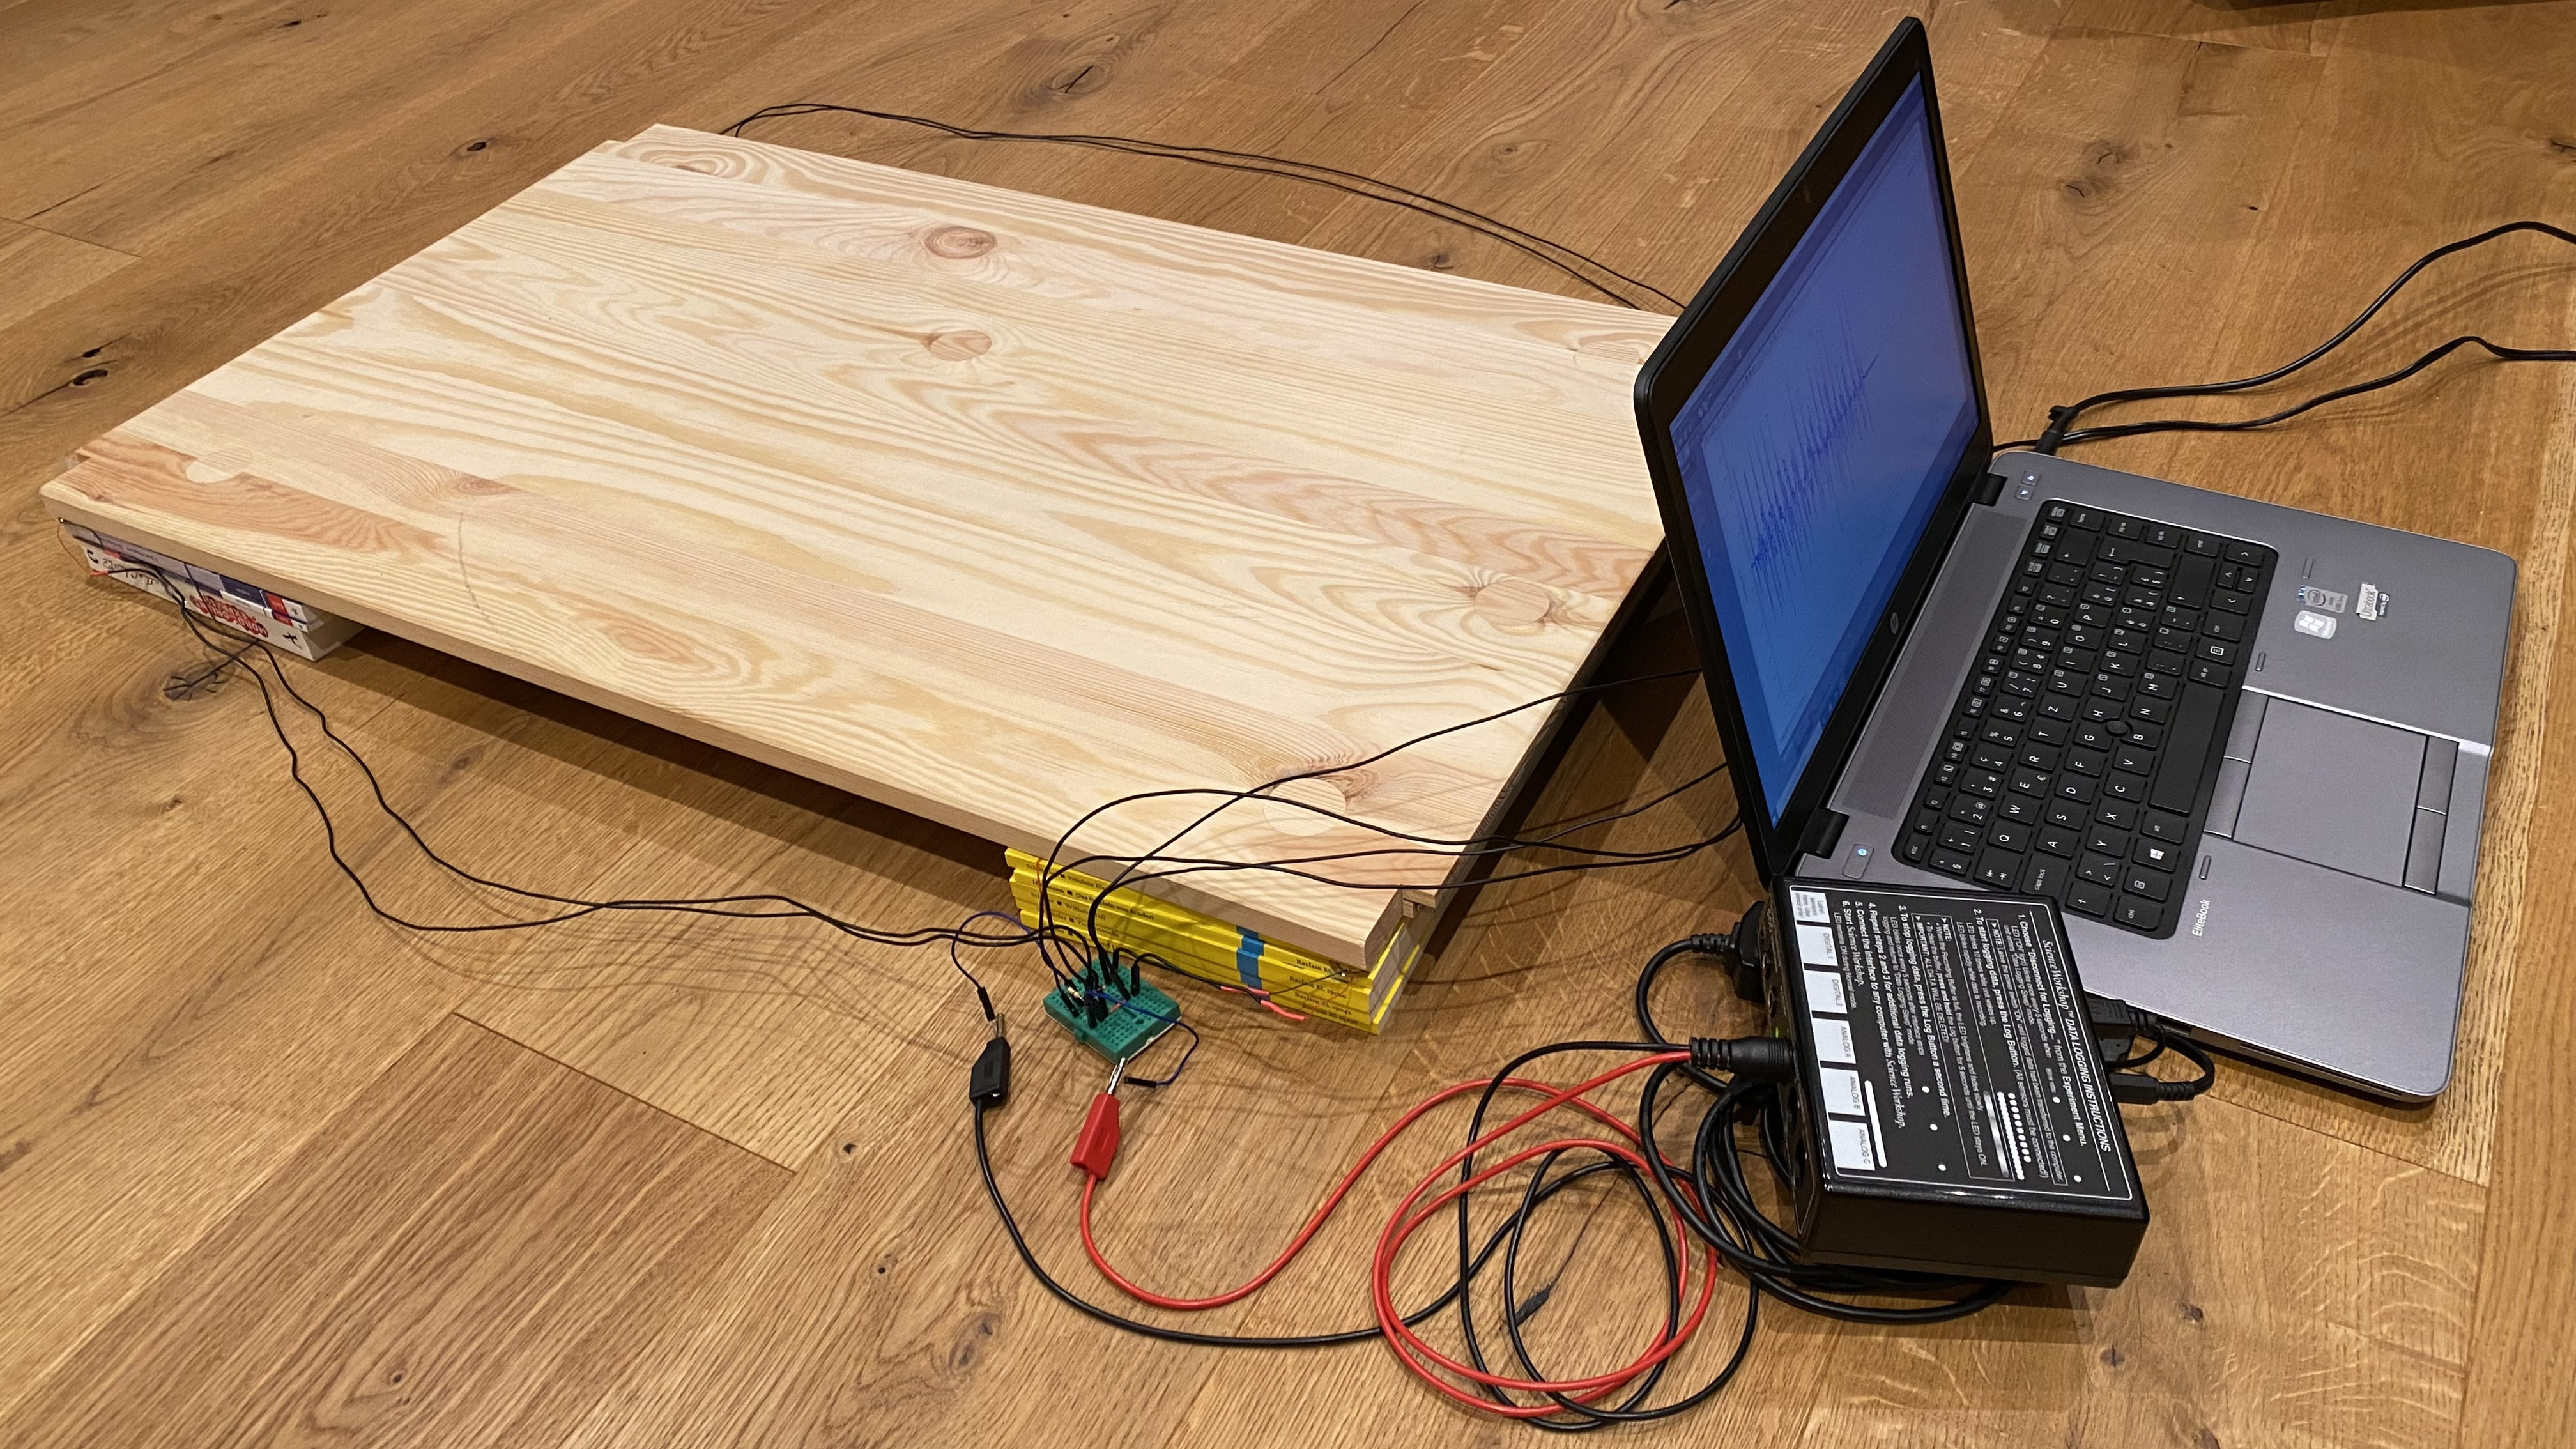
\includegraphics[width=\textwidth]{./Figure_6.jpg}
    \captionof{figure}{Experiment}
    \label{fig:Experiment}
\end{minipage}
\begin{minipage}{0.66\textwidth}
    For the experiment four piezoelectric elements were placed under the corners of a wooden board of dimensions $0.8 \times 0.4 \times 0.02$ m. (Figure \ref{fig:Experiment}) These were then connected to a brad board parallel to a $470k\Omega$ resistor. A voltmeter was connected to the resistor and measured the voltage output while a person was jumping on the wooden board from a height of 20 cm $\pm 1$ cm.\\
\end{minipage}
\begin{minipage}{0.33\textwidth}
    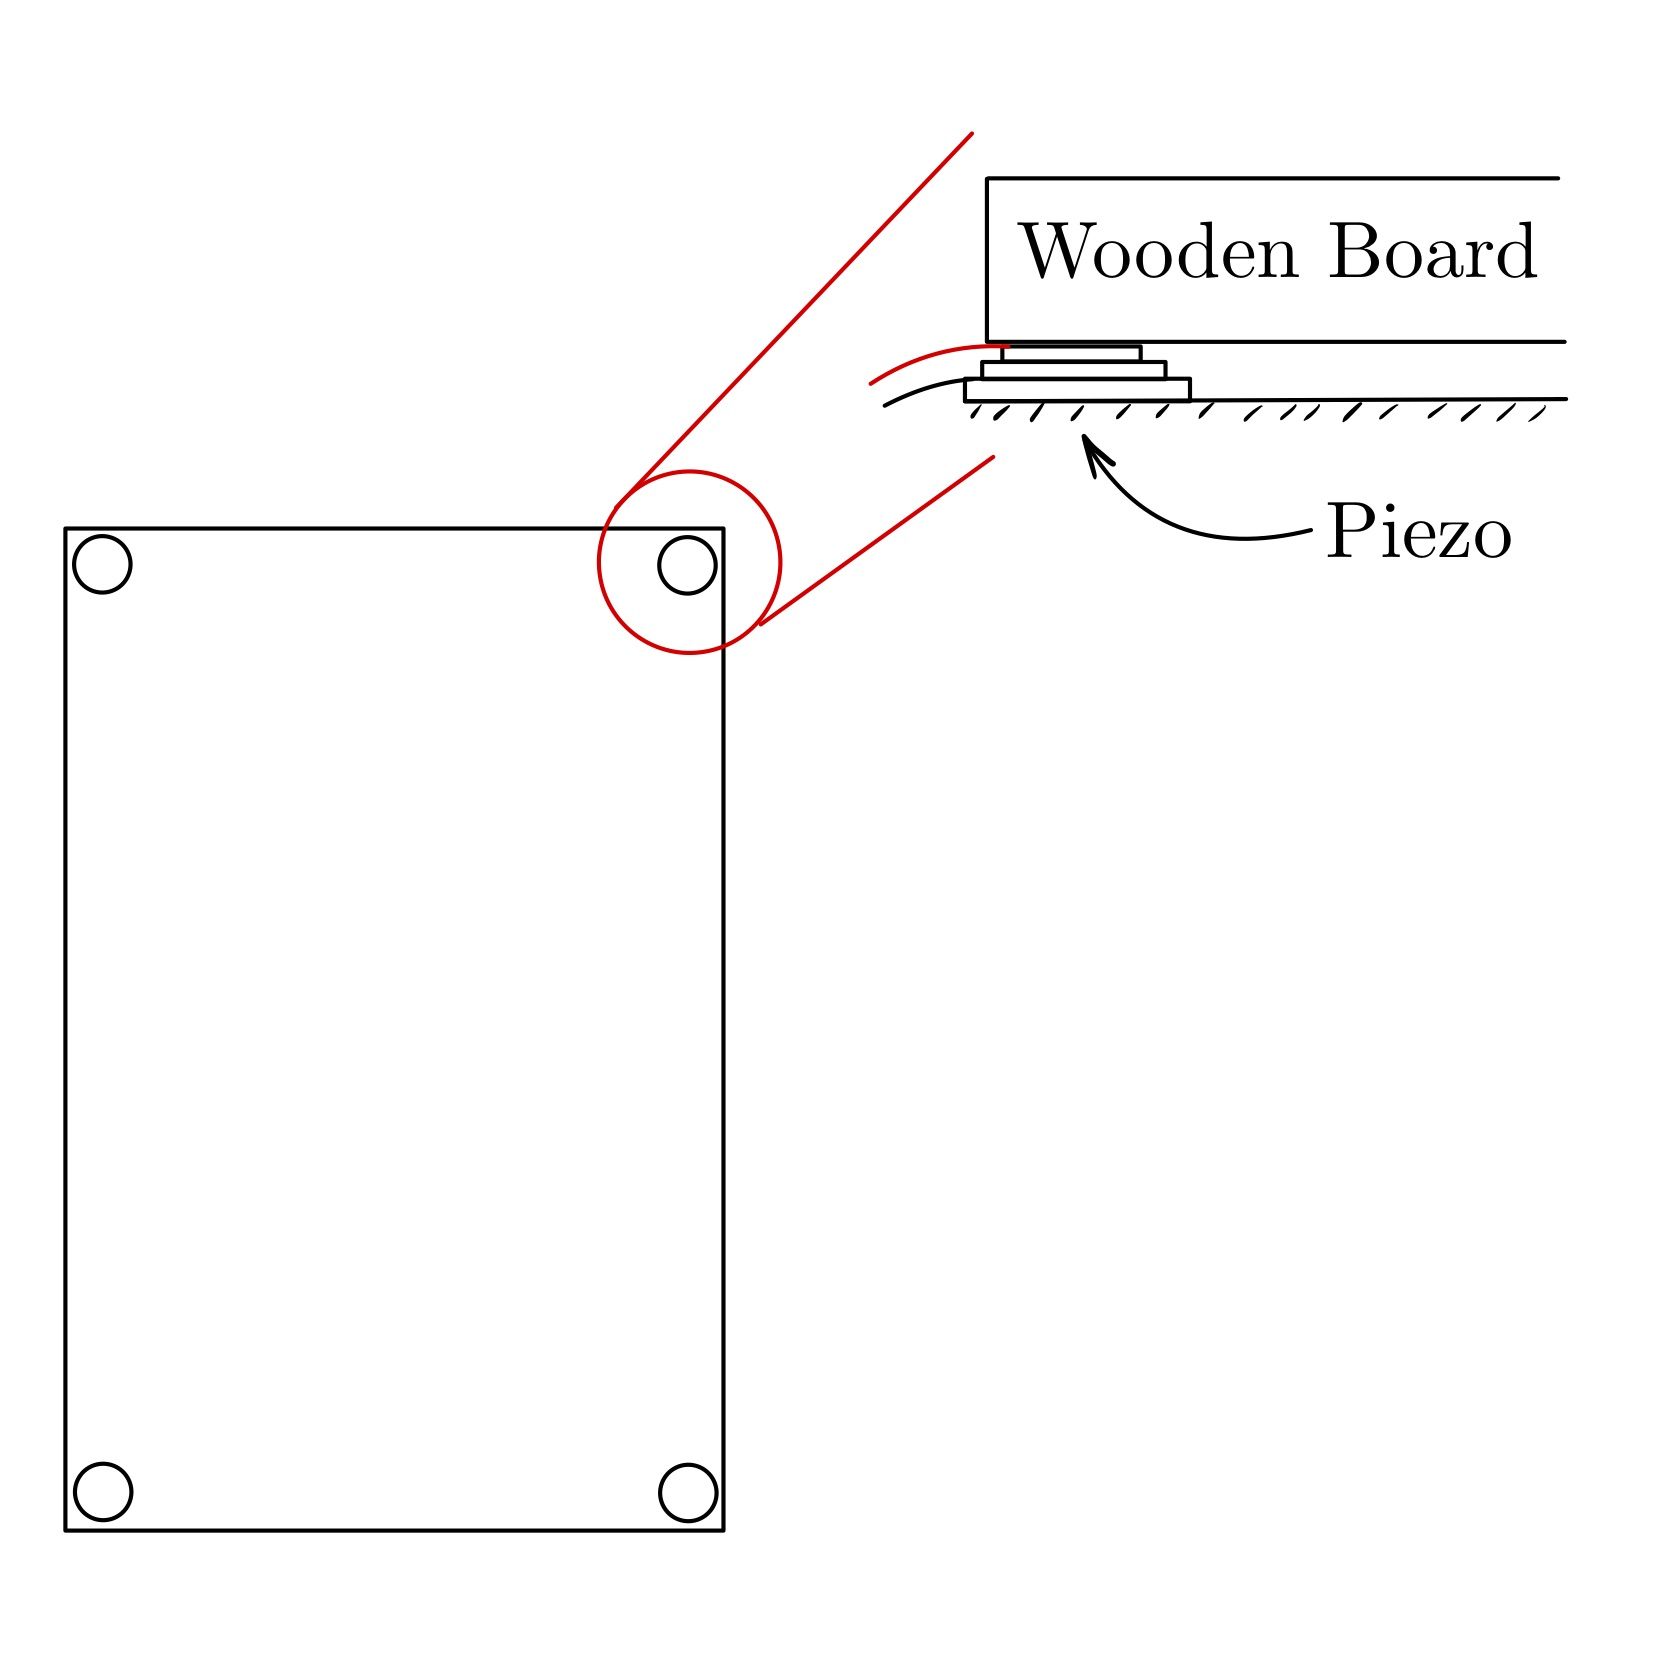
\includegraphics[width=\textwidth]{./Figure_7.jpg}
    \captionof{figure}{Wooden board with piezoelectric elements}
    \label{fig:Wooden board with piezoelectric elements}
\end{minipage}
\begin{minipage}{0.66\textwidth}
    To get an ideal result, the board must be elevated as in Figure \ref{fig:Wooden board with piezoelectric elements}. This ensures an ideal result for the experiment since all the force will be applied onto the four piezo electric elements.\\
\end{minipage}
\begin{minipage}{0.33\textwidth}
    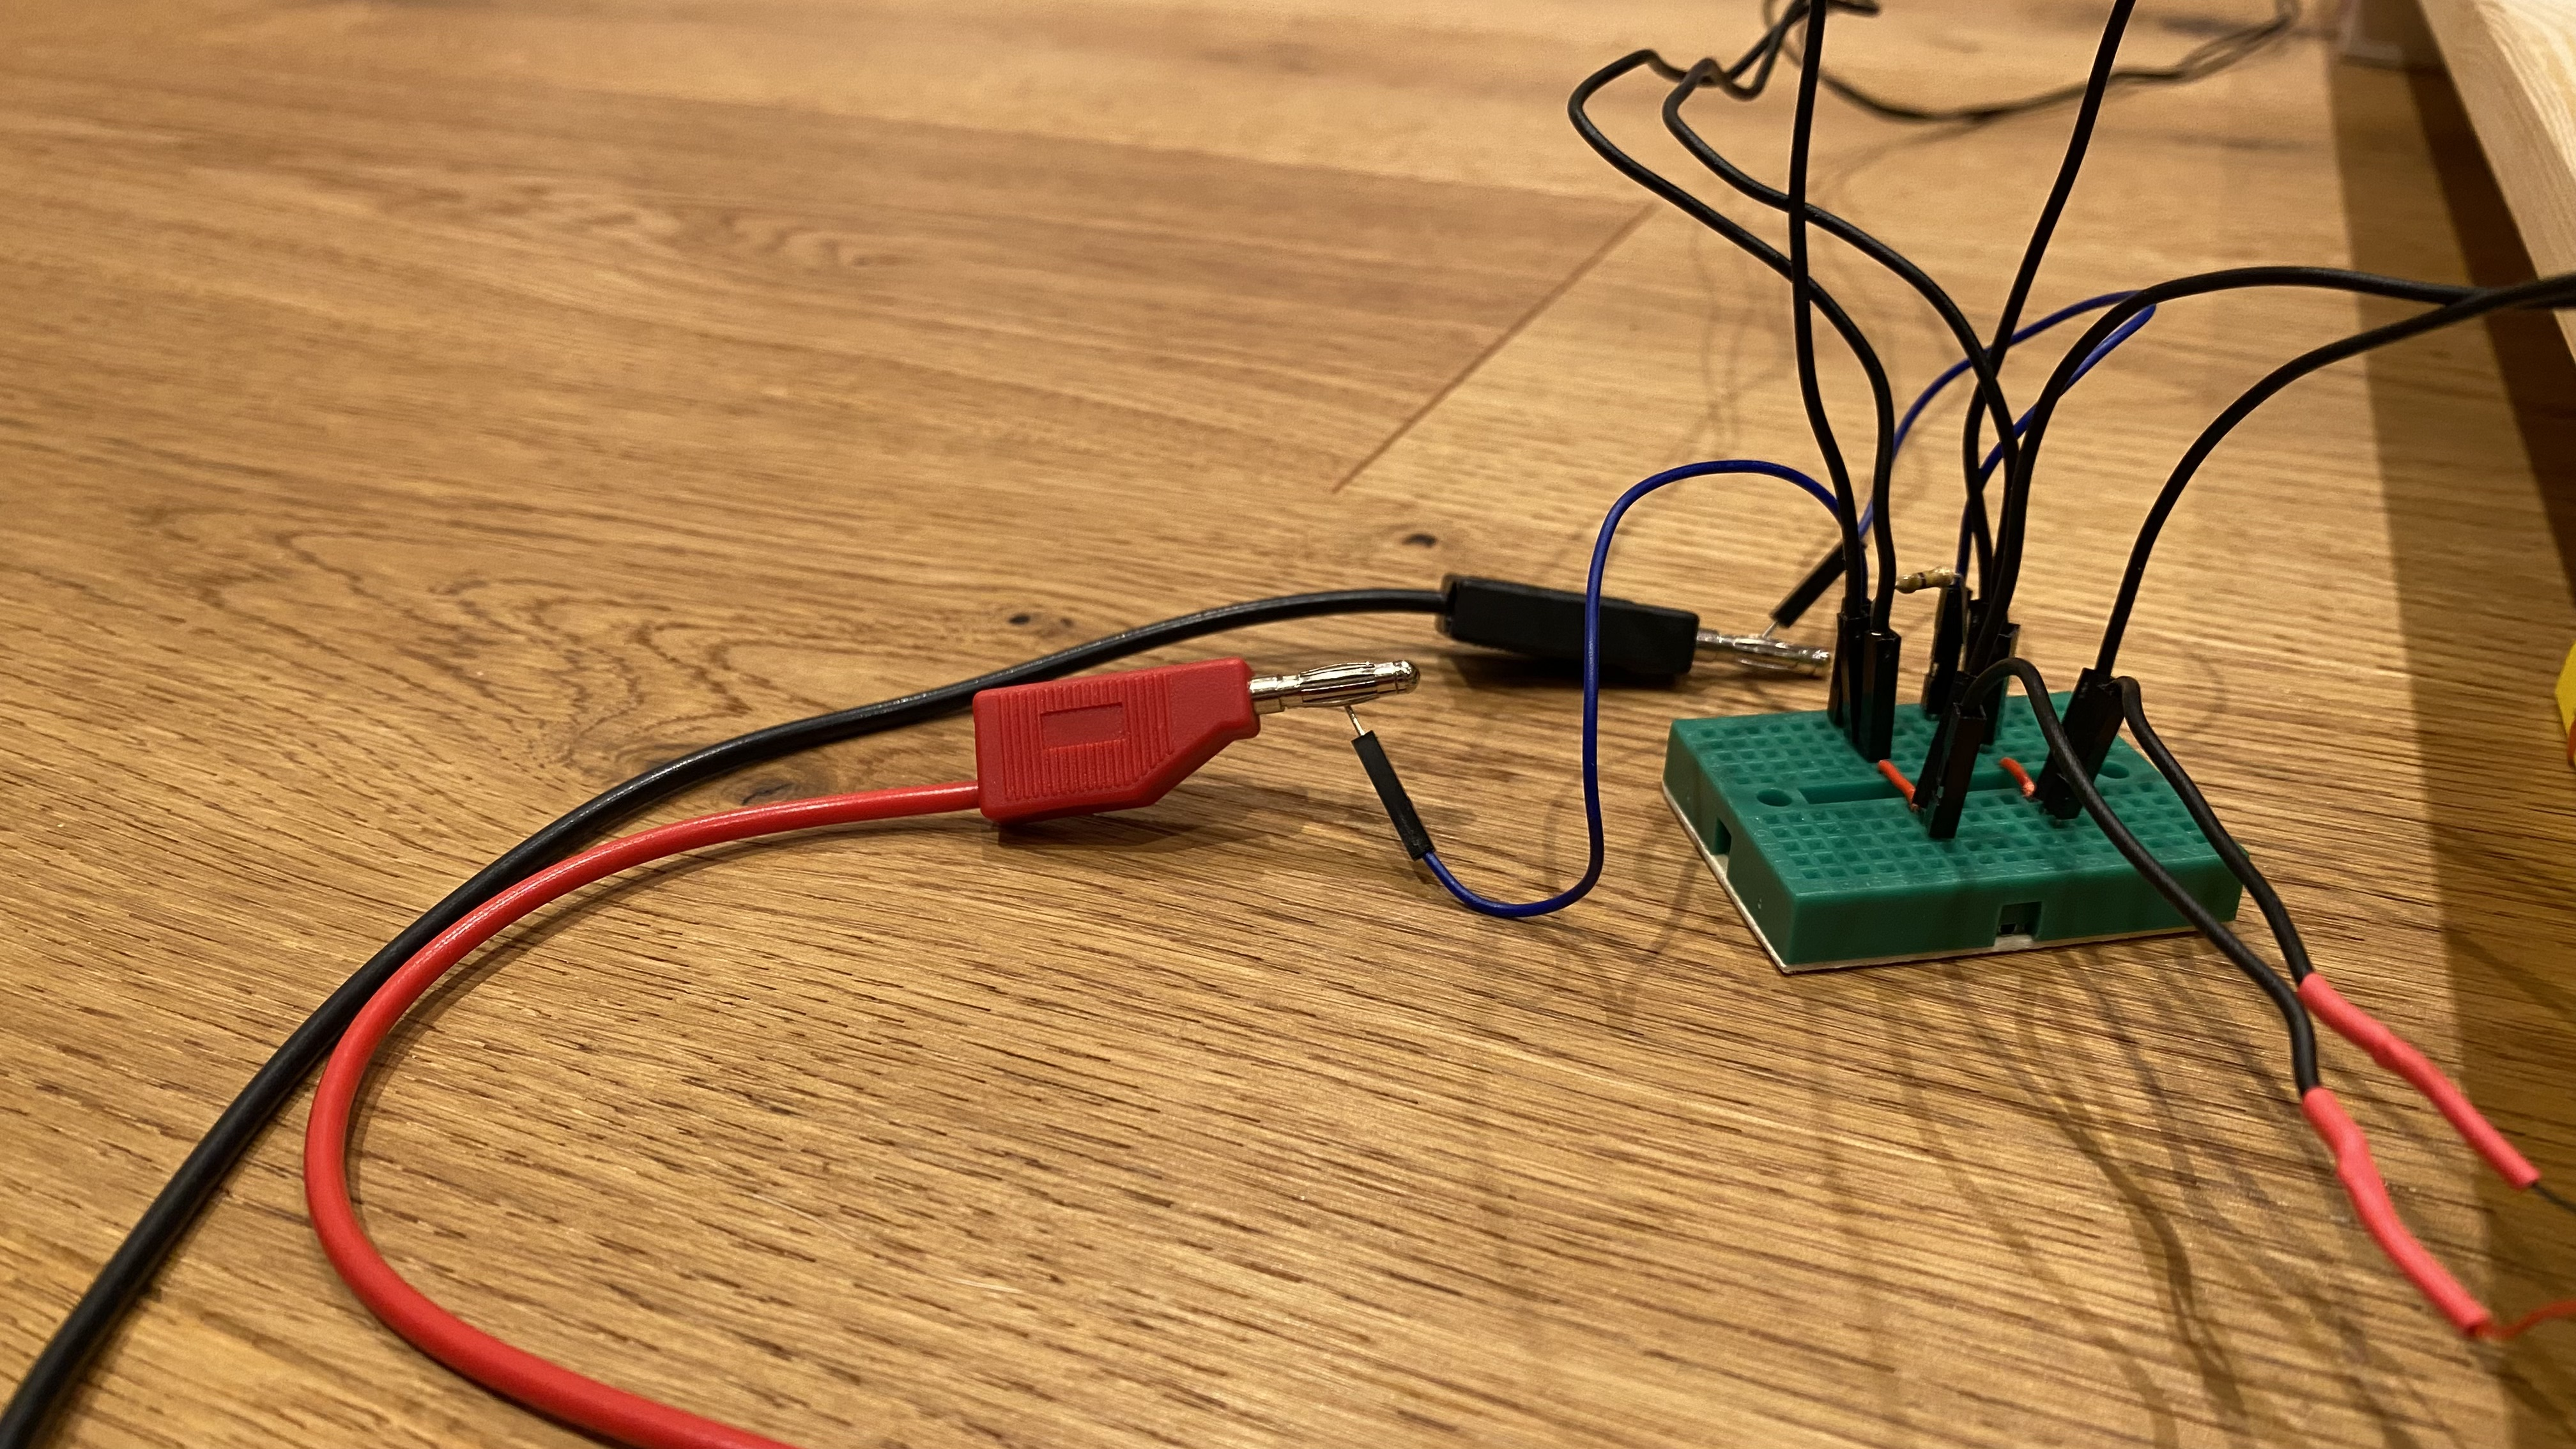
\includegraphics[width=\textwidth]{./Figure_8.jpg}
    \captionof{figure}{Piezoelectric Elements connected in parallel}
    \label{fig:Piezoelectric Elements connected in parallel}
\end{minipage}
\begin{minipage}{0.33\textwidth}
    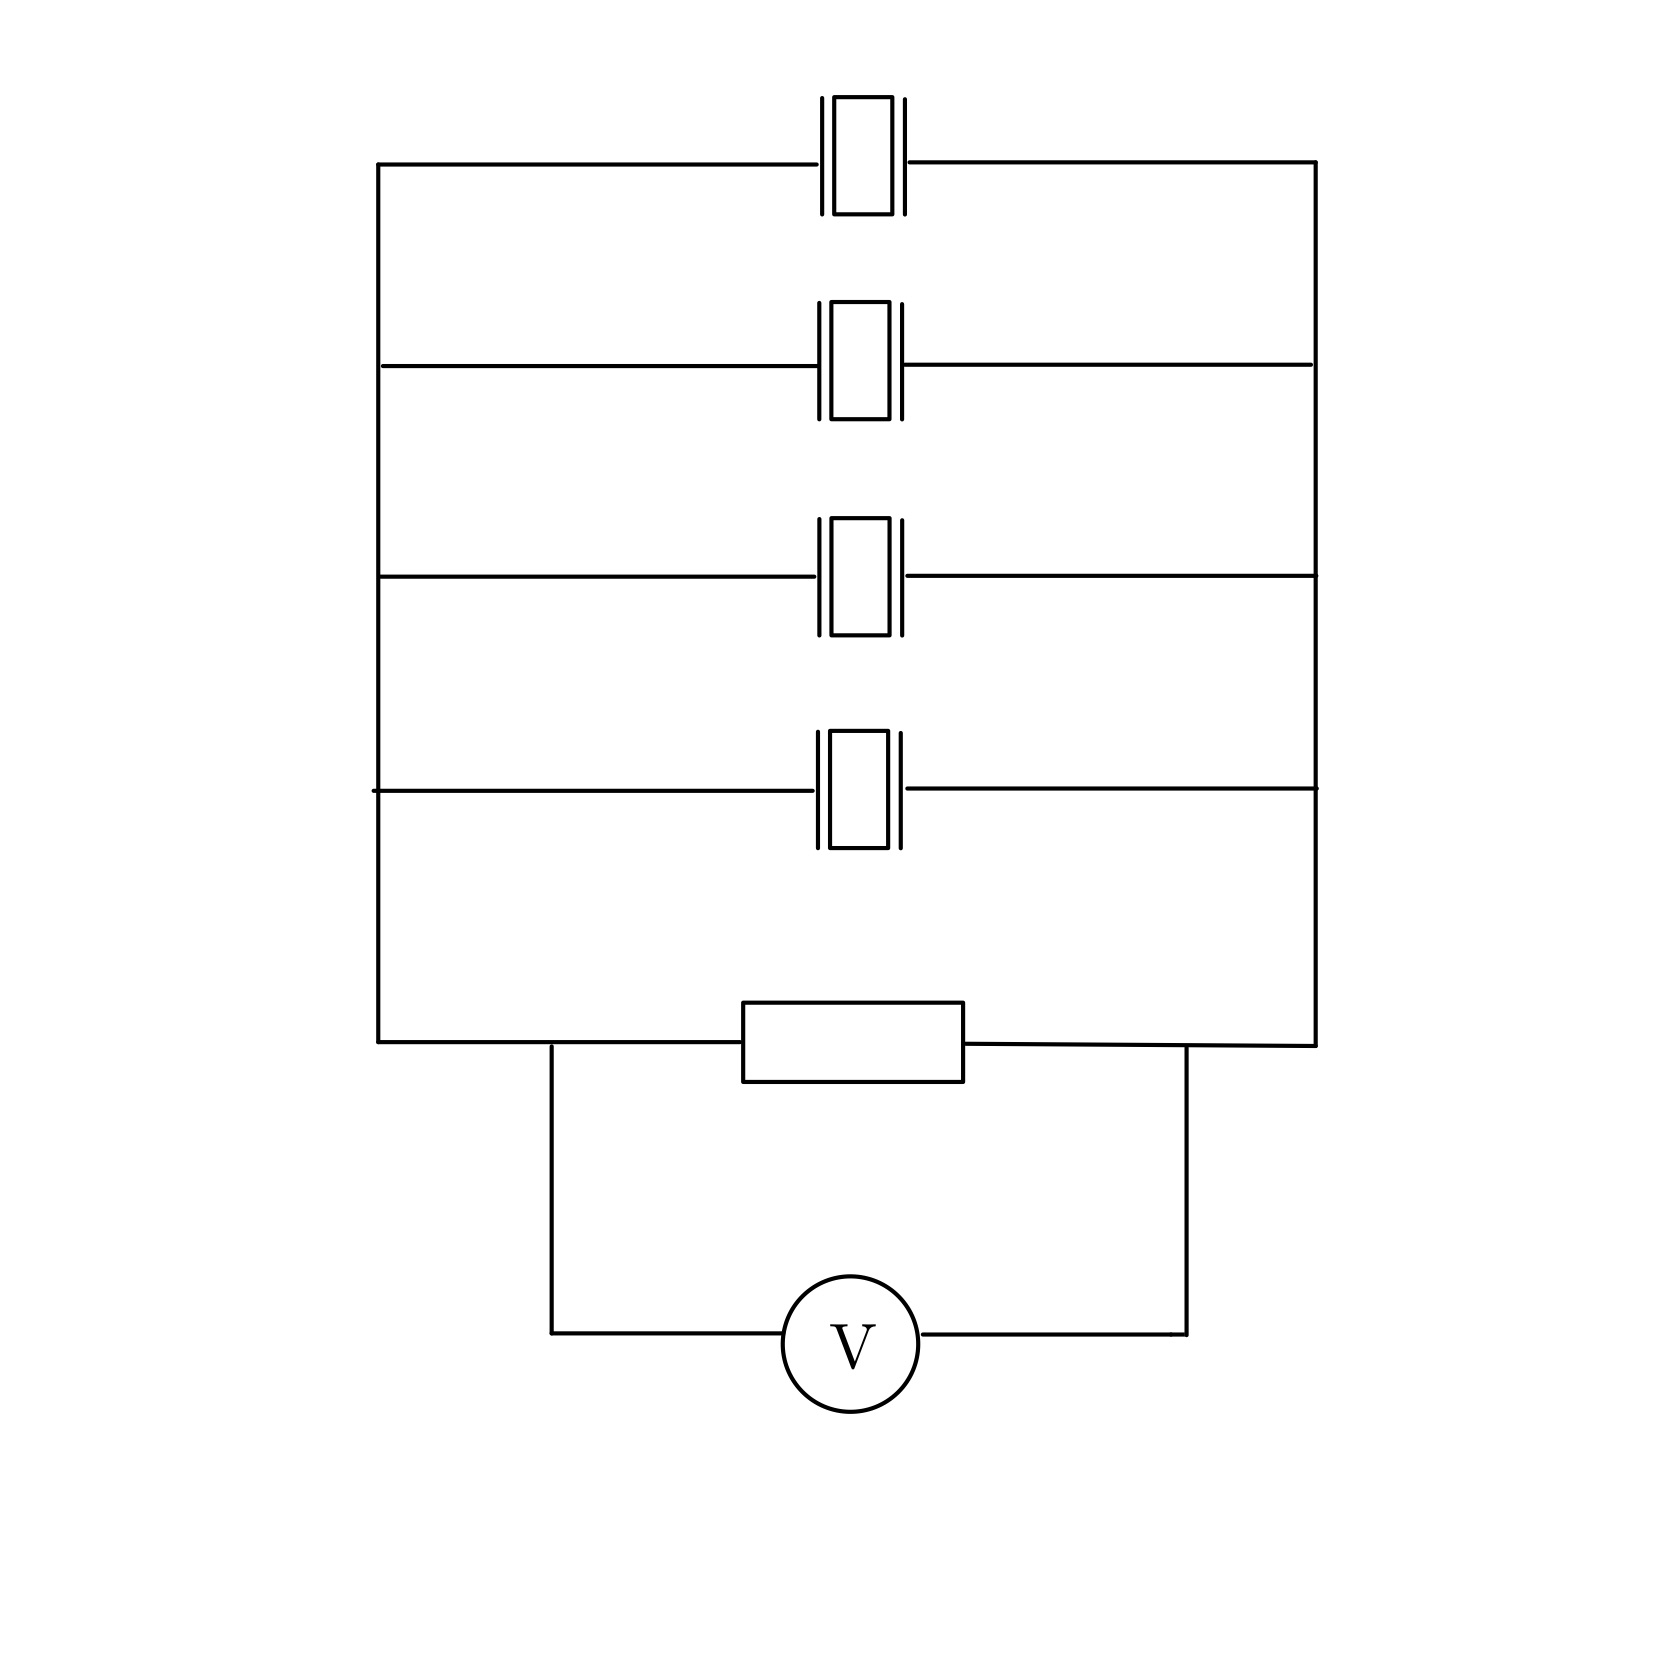
\includegraphics[width=\textwidth]{./Figure_9.jpg}
    \captionof{figure}{Circuit Diagram}
    \label{fig:Circuit Diagram}
\end{minipage}
\begin{minipage}{0.33\textwidth}
    The piezoelectric elements were connected in parallel in addition with a $470k\Omega$ resistor. As represented in Figure \ref{fig:Piezoelectric Elements connected in parallel} and \ref{fig:Circuit Diagram} the voltmeter was then parallel connected to the resistor.\\
\end{minipage}
\begin{minipage}{0.33\textwidth}
    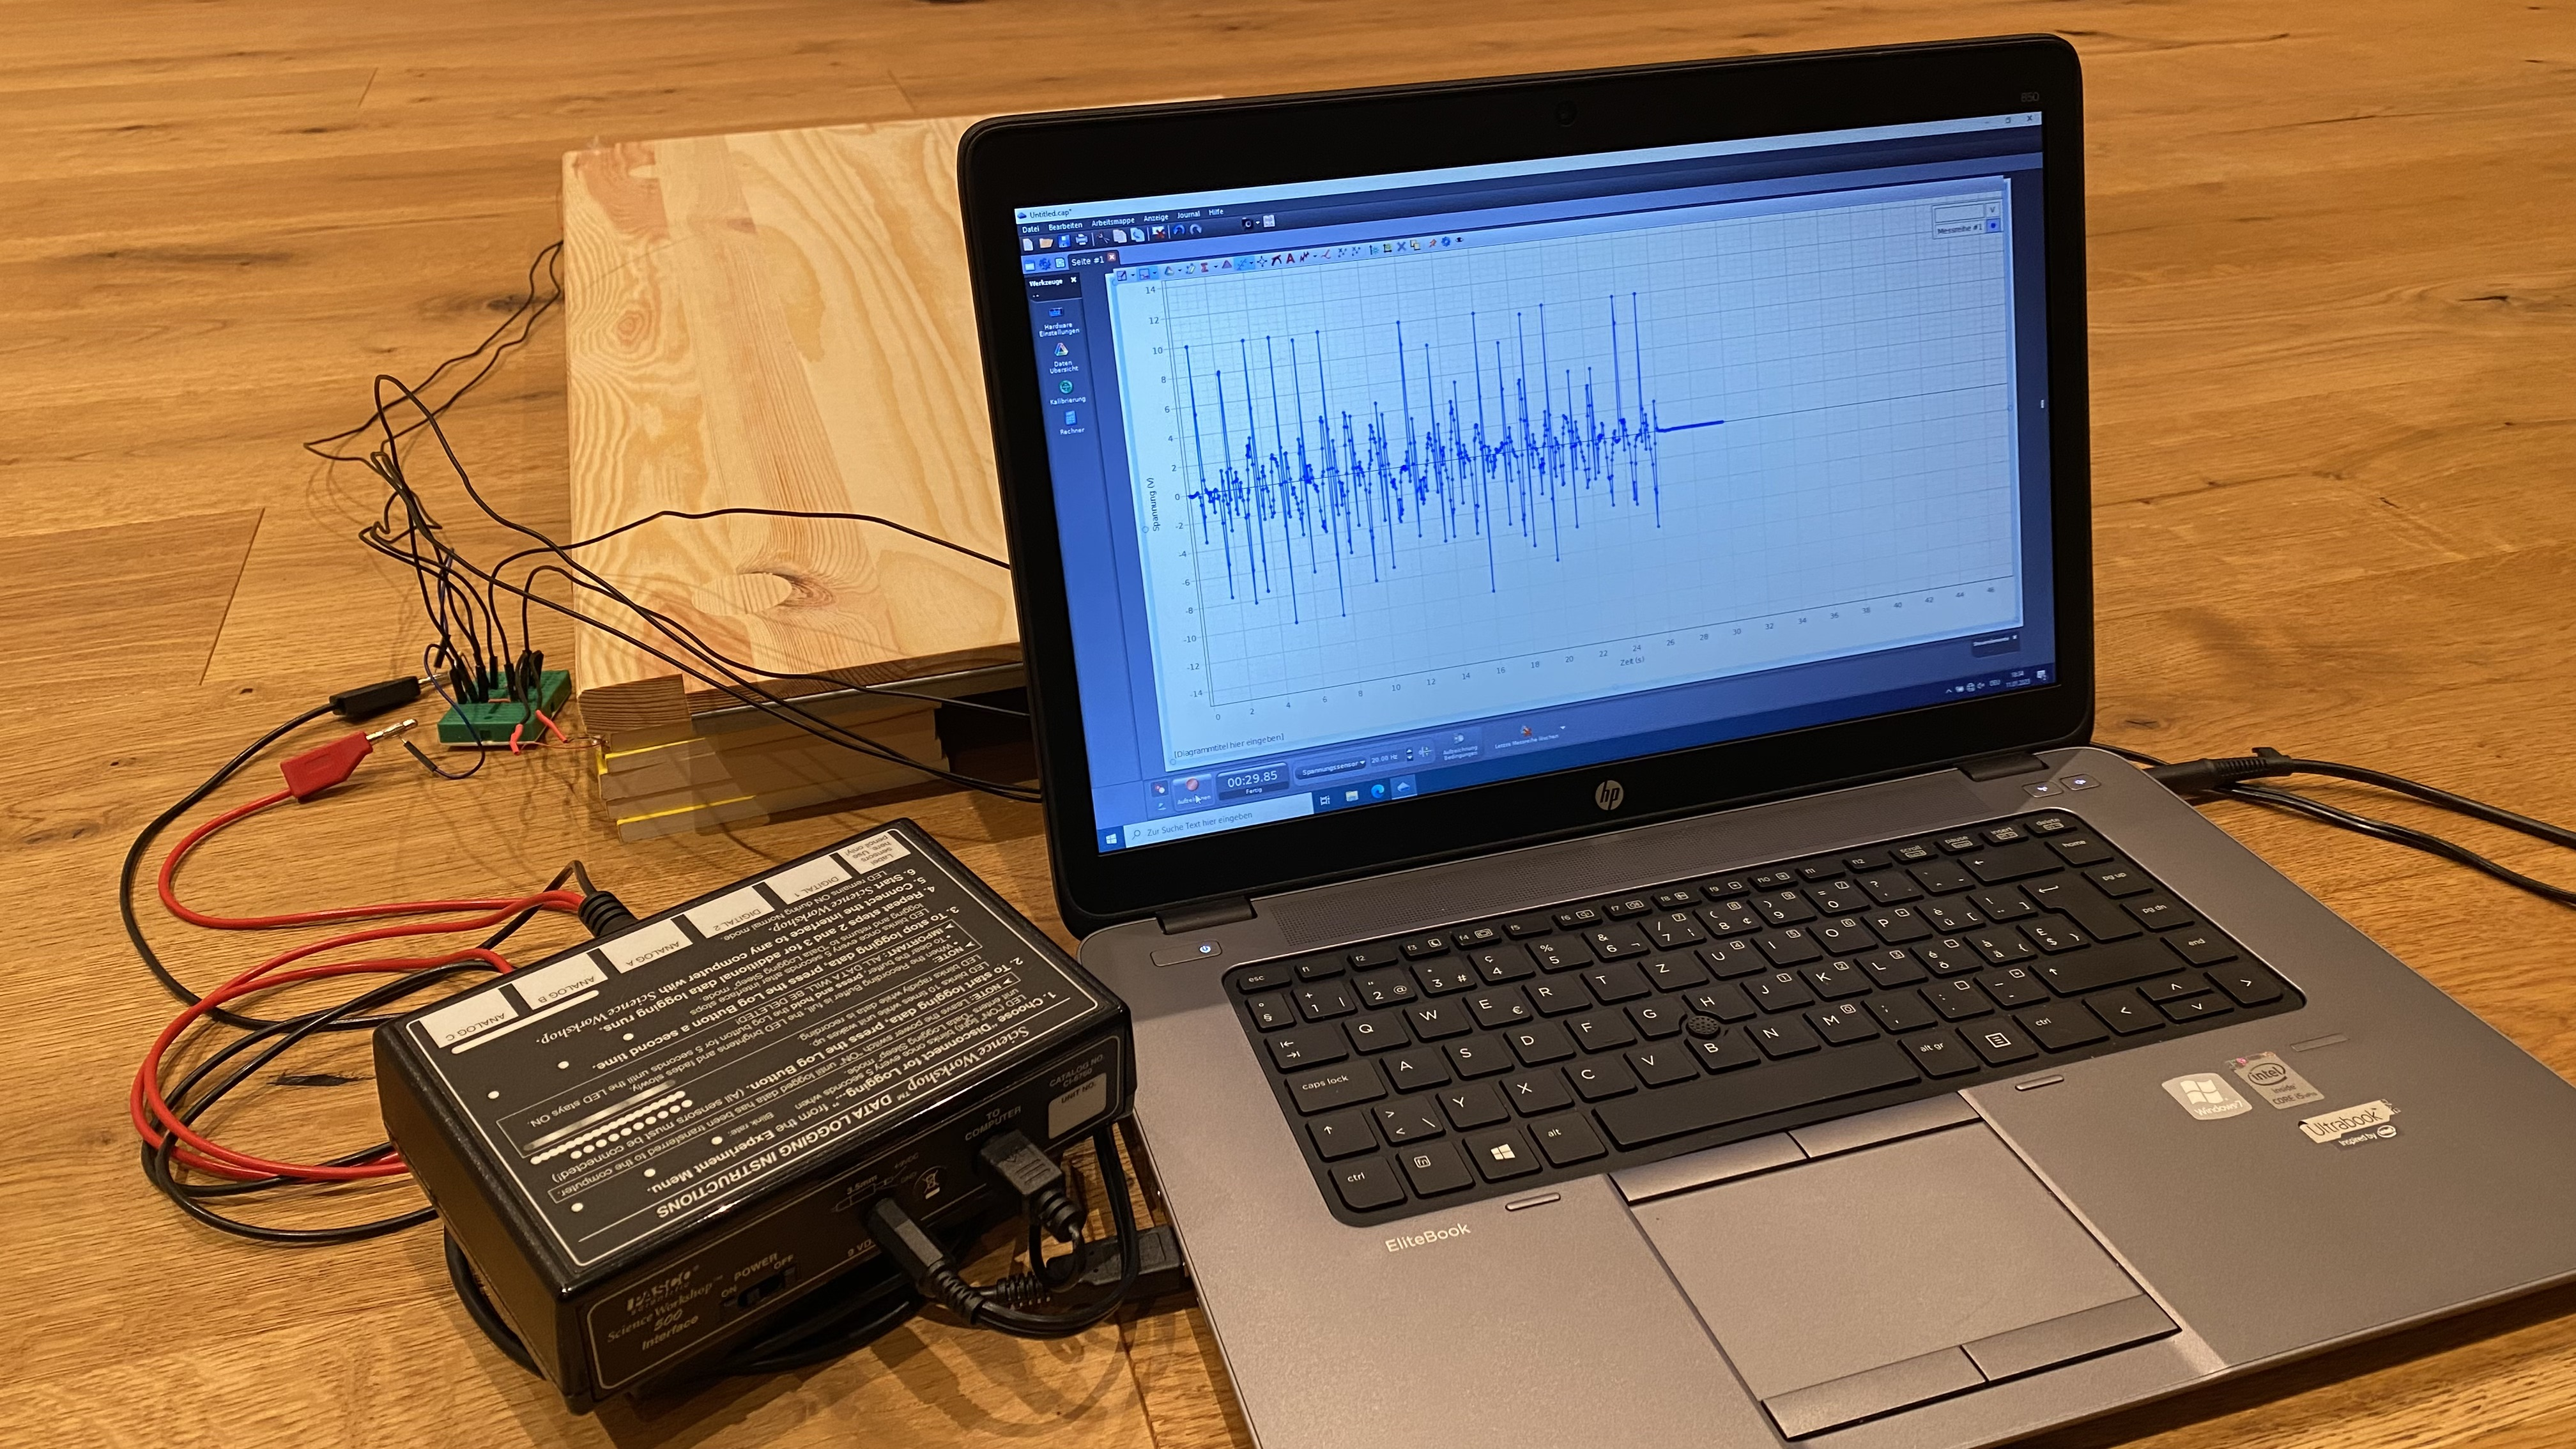
\includegraphics[width=\textwidth]{./Figure_10.jpg}
    \captionof{figure}{Laptop and Pasco Interface 500}
    \label{fig:Laptop and Pasco Interface 500}
\end{minipage}
\begin{minipage}{0.66\textwidth}
    For the measurement, a Pasco 500 Interface was used to measure the voltage. A laptop logged the data and plotted graphs. (Figure \ref{fig:Laptop and Pasco Interface 500})
\end{minipage}
\section{Theoretical Calculation}

The formula $U = g \cdot \frac{F \cdot t}{A}$ can be used to calculate the voltage output of the four piezoelectric elements where $g = 21.3$, $t = 0.00022m$, and $A = 0.000154m^2$. The impact force is estimated to be $730 \pm 2$ N. This results in a voltage of $22.22 \pm 0.06$ V. 
$$
U = g \cdot \frac{F \cdot t}{A}
$$
\begin{equation*}
    \begin{split}
    U & = \frac{U_{\text{max}}+ U_{\text{min}}}{2} \pm \frac{U_{\text{max}}- U_{\text{min}}}{2}\\
    & = 22.22 \pm 0.06 V
    \end{split}
\end{equation*}
For the energy, the formula $E = \frac{1}{2} \cdot F \cdot \frac{F}{k}$ can be used where $F = 730 \pm 2$ $N$ and $k = 10^{10}$ $N/m$. This results in $26.6 \pm 0.000143 \mu J$ which is about $7.4 nWh$.
$$
E = \frac{1}{2} \cdot F \cdot \frac{F}{k}
$$
\begin{equation*}
    \begin{split}
    E & = \frac{E_{\text{max}}+ E_{\text{min}}}{2} \pm \frac{E_{\text{max}}- E_{\text{min}}}{2}\\
    & = 26.6 \pm 0.000143 \mu J = 7.4 nWh
    \end{split}
\end{equation*}

\section{Evaluation of the Measurements}

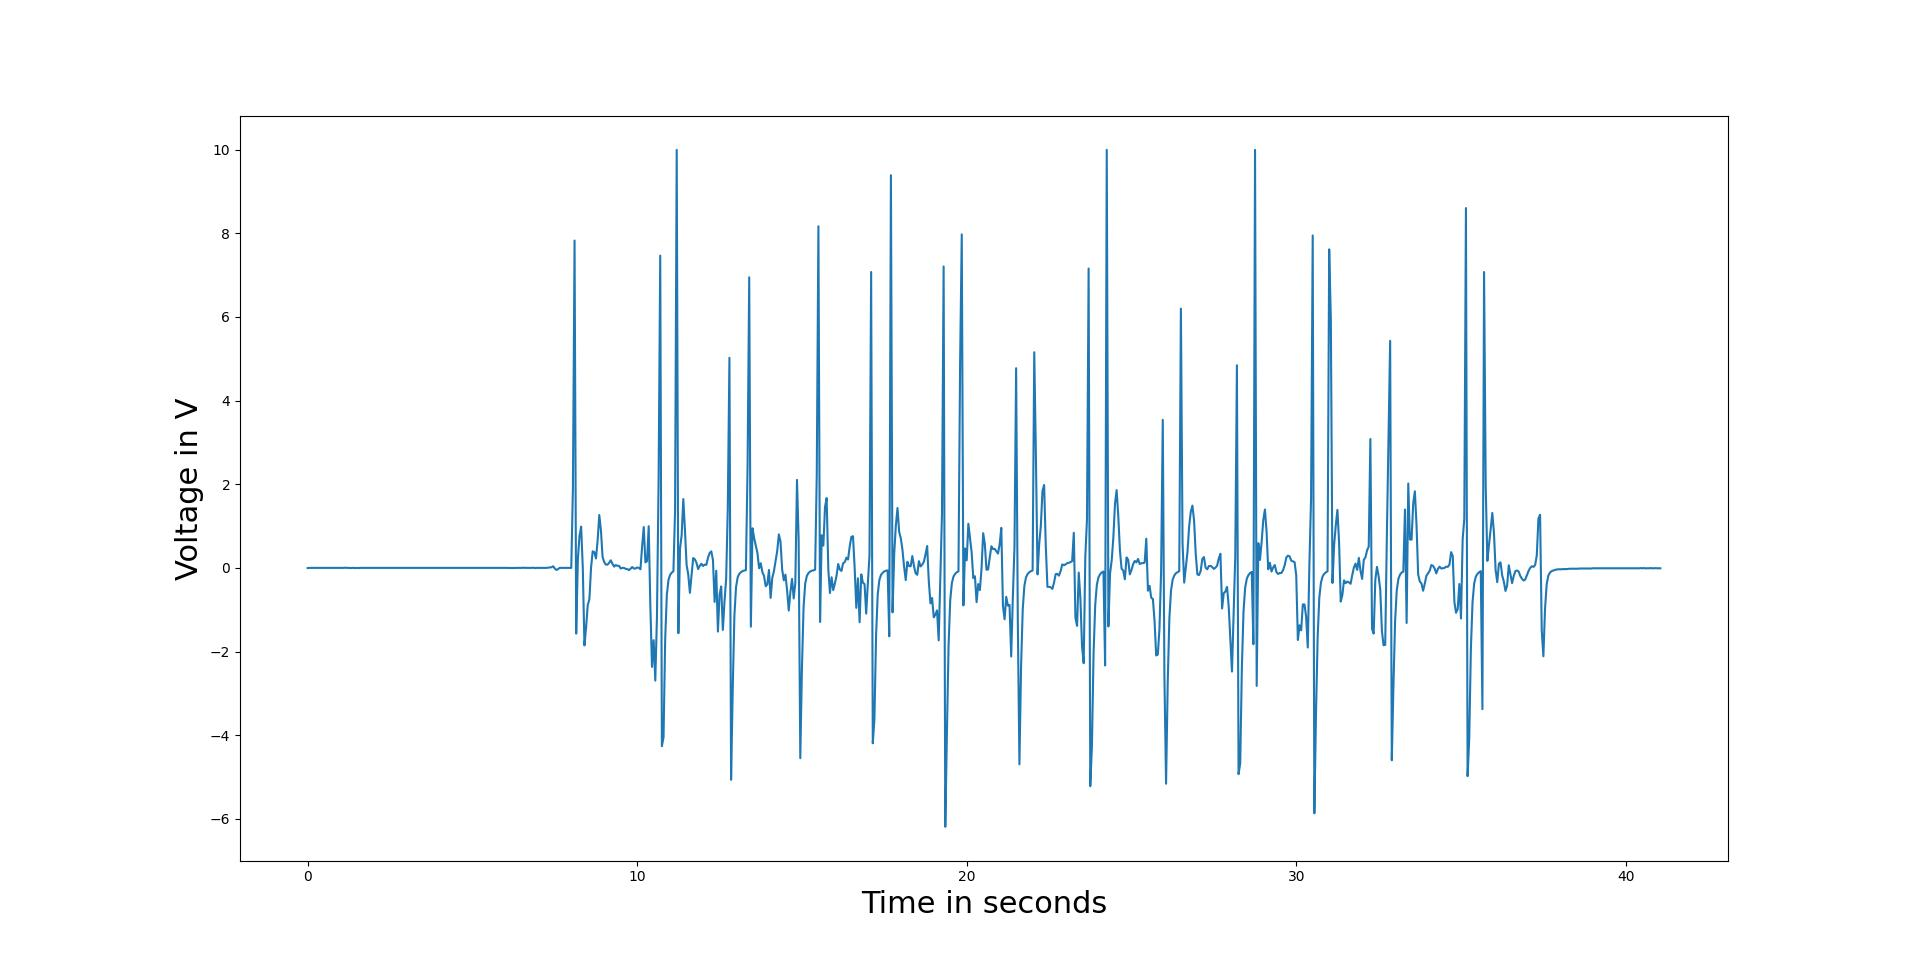
\includegraphics[width=\textwidth]{Figure_11.jpeg}
\captionof{figure}{Voltage Graph of Experiment}
\label{fig:Voltage Graph of Experiment}
\vspace{0.5cm}
When looking at the voltage graph (Figure \ref{fig:Voltage Graph of Experiment}) one can see that the voltage fluctuates between $-6.191 \pm 0.001$ and $9.995 \pm 0.001$ V. This is caused by the quartz expanding after being compressed. Since the quartz obeys the laws of conservation of energy the quartz crystal will not go back to its initial state but will overexpand. This causes the AC voltage. If DC voltage is needed a rectifier has to be used to convert AC into DC voltage.
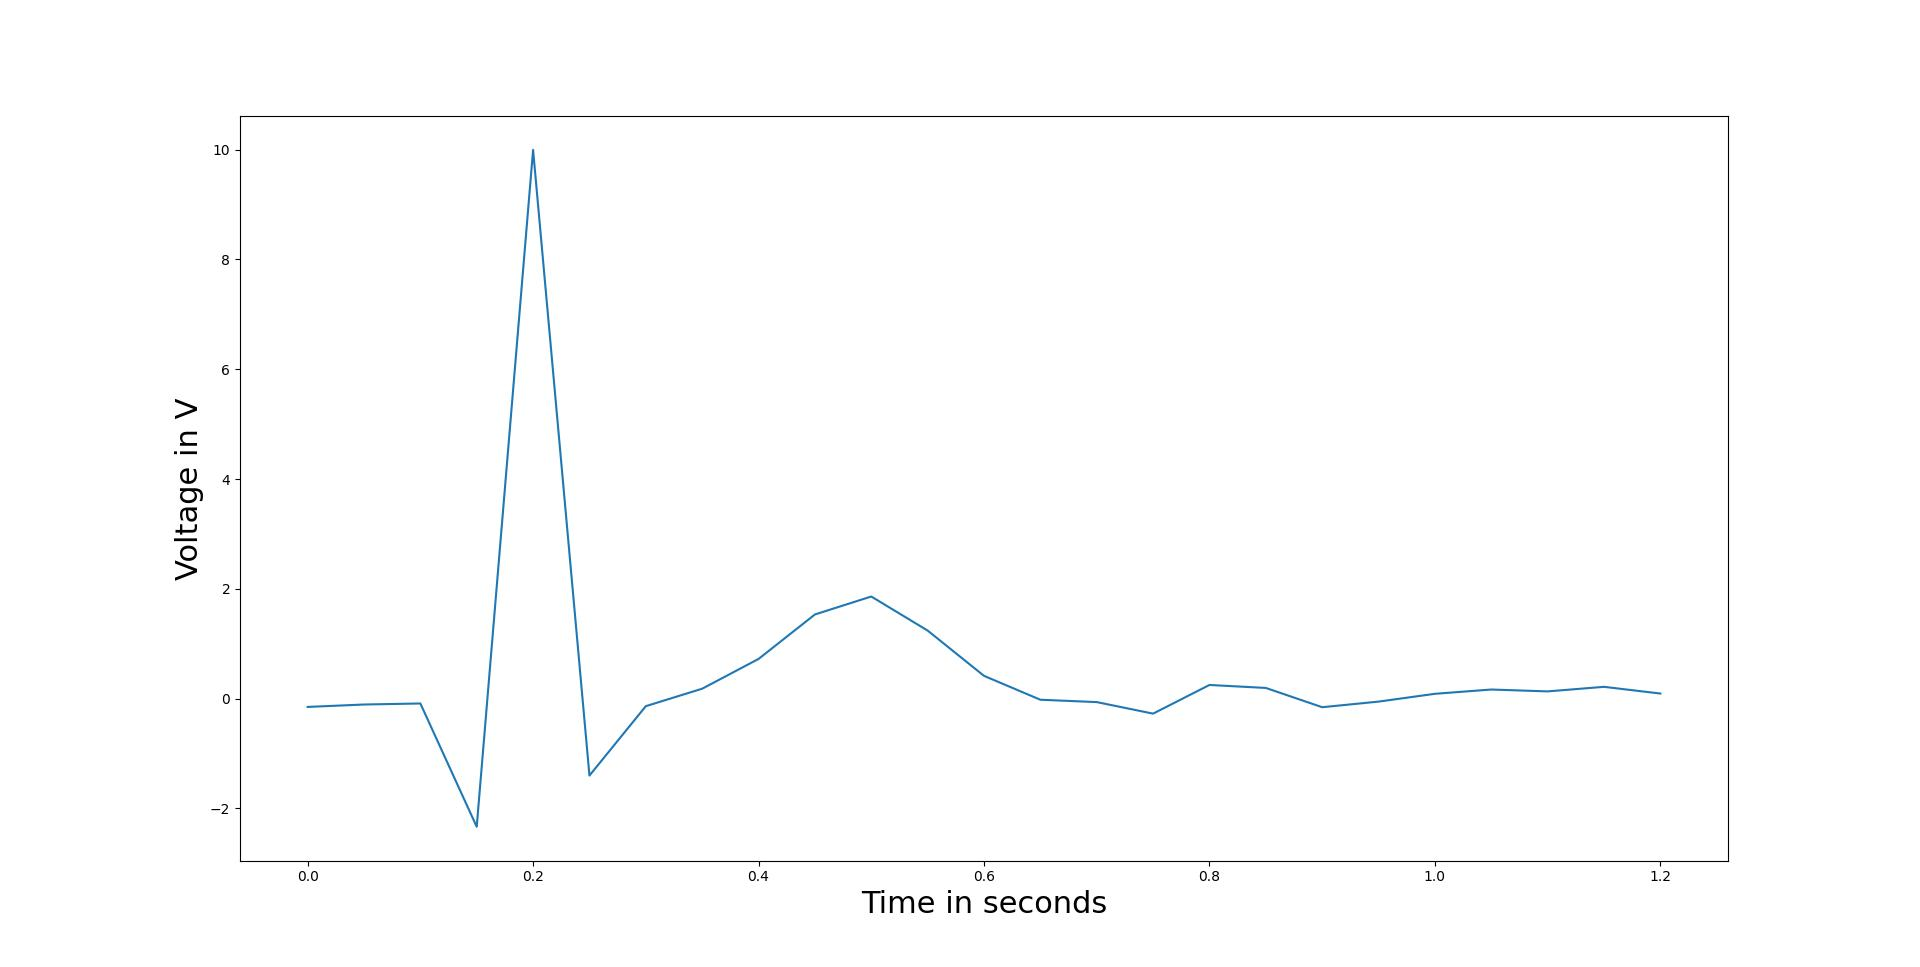
\includegraphics[width=\textwidth]{Figure_12.jpeg}
\captionof{figure}{Section of the Voltage Graph}
\label{fig:Section of the Voltage Graph}
\vspace{0.5cm}
Having a look at Figure \ref{fig:Section of the Voltage Graph} one can see that the piezoelectric element undergoes many different stages. At first the piezoelectric element undergoes a expansion since the weight force is eliminated while jumping up. At the moment of impact, the piezoelectric element is compressed and a voltage can be meassured with its maximum being the peak voltage. Afterwards, the piezoelectric element decompresses going back to its initial state.